




%%
\documentclass[preprint,12pt]{elsarticle}\usepackage[]{graphicx}\usepackage[]{color}
%% maxwidth is the original width if it is less than linewidth
%% otherwise use linewidth (to make sure the graphics do not exceed the margin)
\makeatletter
\def\maxwidth{ %
  \ifdim\Gin@nat@width>\linewidth
    \linewidth
  \else
    \Gin@nat@width
  \fi
}
\makeatother

\definecolor{fgcolor}{rgb}{0.345, 0.345, 0.345}
\newcommand{\hlnum}[1]{\textcolor[rgb]{0.686,0.059,0.569}{#1}}%
\newcommand{\hlstr}[1]{\textcolor[rgb]{0.192,0.494,0.8}{#1}}%
\newcommand{\hlcom}[1]{\textcolor[rgb]{0.678,0.584,0.686}{\textit{#1}}}%
\newcommand{\hlopt}[1]{\textcolor[rgb]{0,0,0}{#1}}%
\newcommand{\hlstd}[1]{\textcolor[rgb]{0.345,0.345,0.345}{#1}}%
\newcommand{\hlkwa}[1]{\textcolor[rgb]{0.161,0.373,0.58}{\textbf{#1}}}%
\newcommand{\hlkwb}[1]{\textcolor[rgb]{0.69,0.353,0.396}{#1}}%
\newcommand{\hlkwc}[1]{\textcolor[rgb]{0.333,0.667,0.333}{#1}}%
\newcommand{\hlkwd}[1]{\textcolor[rgb]{0.737,0.353,0.396}{\textbf{#1}}}%
\let\hlipl\hlkwb

\usepackage{framed}
\makeatletter
\newenvironment{kframe}{%
 \def\at@end@of@kframe{}%
 \ifinner\ifhmode%
  \def\at@end@of@kframe{\end{minipage}}%
  \begin{minipage}{\columnwidth}%
 \fi\fi%
 \def\FrameCommand##1{\hskip\@totalleftmargin \hskip-\fboxsep
 \colorbox{shadecolor}{##1}\hskip-\fboxsep
     % There is no \\@totalrightmargin, so:
     \hskip-\linewidth \hskip-\@totalleftmargin \hskip\columnwidth}%
 \MakeFramed {\advance\hsize-\width
   \@totalleftmargin\z@ \linewidth\hsize
   \@setminipage}}%
 {\par\unskip\endMakeFramed%
 \at@end@of@kframe}
\makeatother

\definecolor{shadecolor}{rgb}{.97, .97, .97}
\definecolor{messagecolor}{rgb}{0, 0, 0}
\definecolor{warningcolor}{rgb}{1, 0, 1}
\definecolor{errorcolor}{rgb}{1, 0, 0}
\newenvironment{knitrout}{}{} % an empty environment to be redefined in TeX

\usepackage{alltt}

%% Use the option review to obtain double line spacing


%% The graphicx package provides the includegraphics command.
\usepackage{graphicx}
%% The amssymb package provides various useful mathematical symbols
\usepackage{amssymb}

\usepackage{lineno}



% \biboptions{}
\IfFileExists{upquote.sty}{\usepackage{upquote}}{}
\begin{document}

\begin{frontmatter}

%% Title, authors and addresses

\title{Pea Plants and Diet Coke: An Experiment}

\author{Jacob Dym and Paul Harmon}

\address{Montana State University}

\begin{abstract}
%% Text of abstract
In order to assess the effects of Diet Coke on the short term growth behavior of plants, we grew pea plants and treated them with different combinations of watering type and plant food. Alaska pea plants were grown in cups treated with a watering regimen consisting of either Diet Coke, diluted Diet Coke, or water. They were also randomized to a combination of either getting plant food upon being planted or not receiving any. A mixed-model was fit to analyze the fixed effects of the two factors while accounting for differences in variation due to the cups and row-blocks in the Randomized block design. Results indicate that pea plants treated with some form of diet coke grew taller than those that were treated with water, regardless of whether or not they received plant food. 
\end{abstract}


\end{frontmatter}

%%
%% Start line numbering here if you want
%%


%% main text
\section{Introduction and Research Questions}

The effect of aspartame, sodium, and other chemical consumption on health outcomes of diet soft-drink consumers has motivated many recent academic studies and garnered attention in the mainstream media. Diet Coke (as well as other brands of diet soda) has been shown to be associated with changes in metabolic behavior and other physiological responses (Veldhuizen, 2017). It has also been linked in longitudinal observational studies to increased risk of stroke. Perhaps unsurprisingly, according to survey analysis performed by Nielsen, diet soda consumption is on the decline, perhaps due to the growing perception that Diet Coke simply is not a healthy choice . But is Diet Coke that bad for consumers? After all, Diet Coke is mostly water (Levitt, 2007). Most scientific work focuses on long-term impacts of soft drink consumption on health via longitudinal studies; however, very little dedicated experimentation has been done to test either its short or long term effects on either humans or plant life. 

The purpose of our experiment, then, is to analyze the short-term effects of Diet Coke on plant growth when used as a substitute for water. The research question addressed by this study is as follows: Does Diet Coke harm the ability of a plant to grow? We posit that since Diet Coke contains ingredients that may be harmful, including aspartame, plants treated exclusively with it instead of water will grow at
a diminished rate relative to those treated with actual water. Based on this, the treatment of interest is whether the plant is watered with pure tap water or a mixture involving Diet Coke. The treatments of this factor are:

\begin{itemize}
\item Diet Coke
\item 22 percent Diet Coke Dilution
\item Tap water (Control)
\end{itemize}

We are also interested in the effect of plant food,  especially whether or not the effect of Diet Coke is modified by the presence or absence of plant food.  It seems possible that the Diet Coke could react differently with soil enriched with plant food than in would with soil that was not enriched at all. 

\begin{itemize}
\item Plant Food (administered at planting)
\item No plant food
\end{itemize}

Previous research has been done on the effect of different types of watering substances on pea plant growth. Work done by Roland et al (2013) found significant differences in pea plant heights when comparing Vitamin Water treatments to an untreated watering regime. Similarly, work by Slutzky et al (2003) found significant differences between pea-plant heights after treatment with unspecified Diet soda, Water, ibuprofen, and sparkling water regimes. However, little appears to have been done to specifically assess the effect of Diet Coke specifically, nor has there been much progress on the assessment of an interaction between presence of plant food and watering type.   




\section{Methods}
\subsection{Experimental Design}

\subsection{Data}


\section{Results and Analysis}
\subsection{Exploratory Analysis}
\begin{knitrout}
\definecolor{shadecolor}{rgb}{0.969, 0.969, 0.969}\color{fgcolor}\begin{figure}
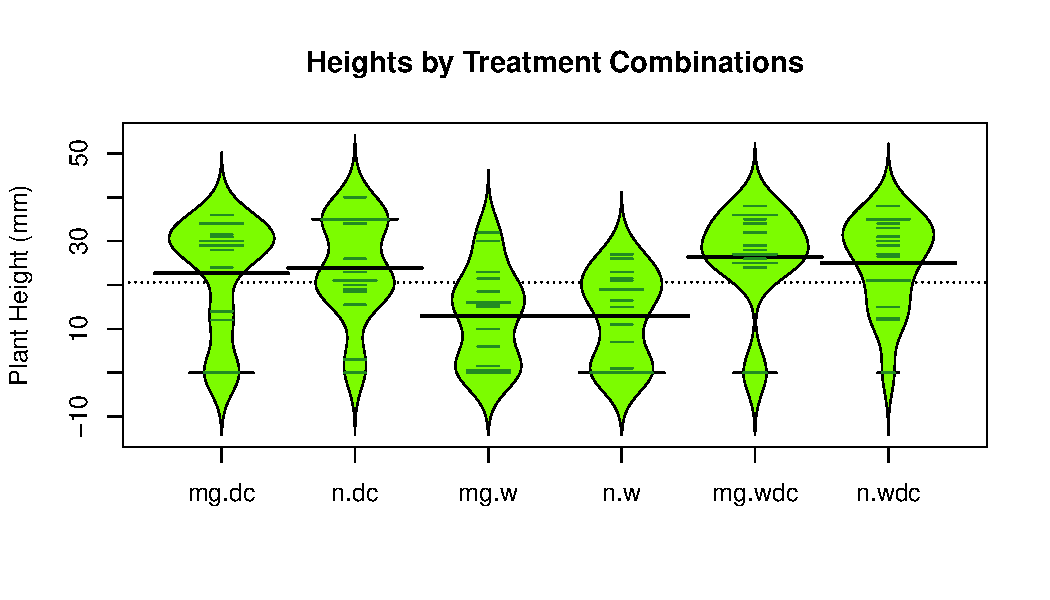
\includegraphics[width=\maxwidth]{figure/eda-1} \caption[Germination rates by treatment group]{Germination rates by treatment group.}\label{fig:eda}
\end{figure}


\end{knitrout}




\subsection{Germination Rates}
Before we could do any statistical analysis of the pea plants, we had to determine that the treatment was not related to the germination probability for a given plant. Overall, 14 of the 82 (15 percent) of the pea plants failed to germinate. 
\begin{knitrout}
\definecolor{shadecolor}{rgb}{0.969, 0.969, 0.969}\color{fgcolor}\begin{figure}
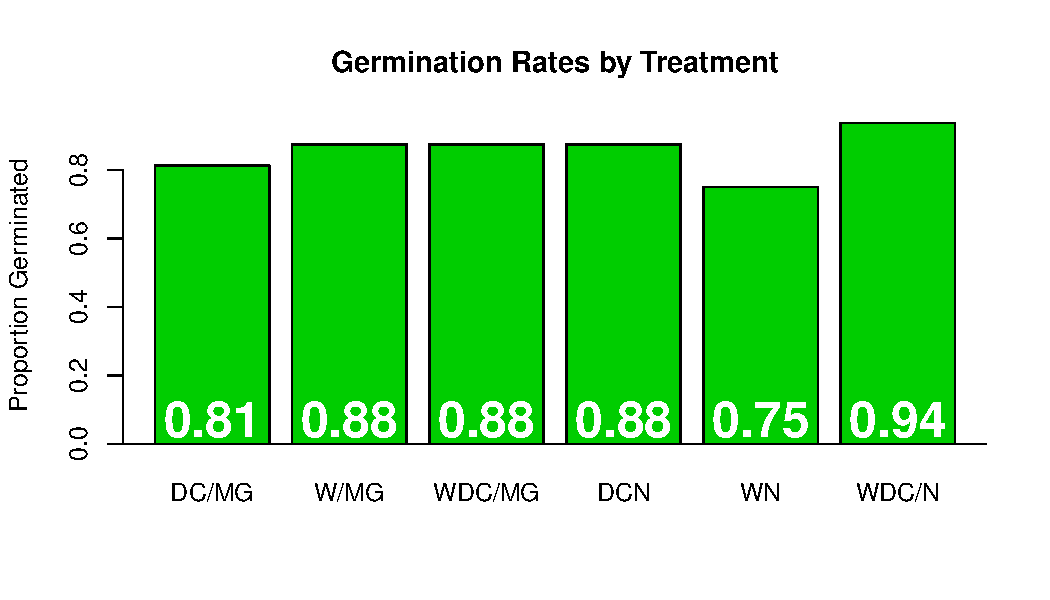
\includegraphics[width=\maxwidth]{figure/germination_rates-1} \caption[Germination rates by treatment group]{Germination rates by treatment group.}\label{fig:germination_rates}
\end{figure}


\end{knitrout}

Since we did not find strong evidence supporting a relationship between germination probability and treatment, we treated the non-germinated plants as unobserved data in the analysis. 



\subsection{Regression Results}

\begin{knitrout}
\definecolor{shadecolor}{rgb}{0.969, 0.969, 0.969}\color{fgcolor}\begin{kframe}
\begin{alltt}
\hlstd{lmer2} \hlkwb{<-} \hlkwd{lmer}\hlstd{(Height} \hlopt{~} \hlstd{TrtCoke} \hlopt{*} \hlstd{PF} \hlopt{+} \hlstd{(}\hlnum{1}\hlopt{|}\hlstd{Block)} \hlopt{+} \hlstd{(}\hlnum{1}\hlopt{|}\hlstd{Cup_Rand),} \hlkwc{data} \hlstd{= pea)}
\end{alltt}


{\ttfamily\noindent\bfseries\color{errorcolor}{\#\# Error in lmer(Height \textasciitilde{} TrtCoke * PF + (1 | Block) + (1 | Cup\_Rand), data = pea): could not find function "{}lmer"{}}}\begin{alltt}
\hlkwd{summary}\hlstd{(lmer2)}
\end{alltt}


{\ttfamily\noindent\bfseries\color{errorcolor}{\#\# Error in summary(lmer2): object 'lmer2' not found}}\begin{alltt}
\hlkwd{Anova}\hlstd{(lmer2,} \hlkwc{type} \hlstd{=} \hlstr{"II"}\hlstd{)}
\end{alltt}


{\ttfamily\noindent\bfseries\color{errorcolor}{\#\# Error in Anova(lmer2, type = "{}II"{}): could not find function "{}Anova"{}}}\begin{alltt}
\hlkwd{plot}\hlstd{(}\hlkwd{allEffects}\hlstd{(lmer2))}
\end{alltt}


{\ttfamily\noindent\bfseries\color{errorcolor}{\#\# Error in allEffects(lmer2): object 'lmer2' not found}}\end{kframe}
\end{knitrout}



\section{Discussion}






\end{document}
